\documentclass[journal]{IEEEtran}
\usepackage{graphicx} % Required for inserting images
\usepackage{amsmath} % For \text in math mode
\usepackage{float}
\usepackage{hyperref}
\usepackage{algorithm}
\usepackage{algpseudocode}
\usepackage{amssymb}
\usepackage{booktabs}
\usepackage{siunitx}
\usepackage{tikz}
\usepackage{adjustbox}
\usepackage{multirow}
\usepackage{enumitem}

\usepackage{cleveref}
\crefname{section}{Section}{Sections}
\crefname{figure}{Fig.}{Figs.}
\crefname{table}{Table}{Tables}
% \crefname{subsection}{Subsection}{Subsections}

\usetikzlibrary{arrows.meta, positioning}

\newtheorem{remark}{Remark}

\title{FASTT: Feature-Adaptive Speech-to-Text Model Selection}
\author{Huseyin~Karaca$^{*}$,
        A.~Samil~Namli$^{*}$, 
        and Suleyman S.~Kozat,~\IEEEmembership{Senior~Member,~IEEE}
\thanks{$^{*}$H. Karaca and A. S. Namli contributed equally to this work.}
\thanks{H. Karaca, A. S. Namli, and S. S. Kozat are with Bilkent University, Ankara, Turkiye. H. Karaca and A. S. Namli are also with Turk Telekom, Ankara, Turkiye (e-mails: \{huseyin.karaca, samil.namli\}@bilkent.edu.tr; kozat@ee.bilkent.edu.tr).}%
\thanks{This work is supported by The Scientific and Technological Research Council of Turkiye (TUBITAK) 1515 Frontier R\&D Laboratories Support Program for Turk Telekom 6G R\&D Lab under project number 5249902, and by the TUBITAK 2210-A program.}%
}
\date{}

\begin{document}
    \maketitle

    \begin{abstract}
    Existing approaches to automatic speech recognition (ASR) either rely on a single speech-to-text (STT) model or combine multiple models through computationally expensive ensemble techniques, leading to suboptimal trade-offs between accuracy and efficiency across diverse acoustic conditions. Since different STT models exhibit complementary strengths, selecting the most suitable model for each input can significantly improve transcription accuracy. He, we introduce FASTT, a feature-adaptive STT selection framework that learns to select the most appropriate pretrained STT expert for each utterance. FASTT jointly learns a task-aligned feature transformation and a lightweight selection function based on acoustic and embedding-derived features, and is trained by directly minimizing a cumulative transcription-error objective. Since in an end to end manner, we learn both the features that best distinguish between S2T models as well as the selection algorithm based on the final cumulative error, FASTT consistently outperforms static selection and standard routing methods. Our experiments, over multiple challenging datasets shows that FASTT achieves up to 8\% relative WER reduction. End-to-end FASTT is approximately 23\% faster on average than classical feature selection methods. Furthermore, we provide convergence guarantees showing that the proposed training procedures converge to first-order stationary points under mild conditions, ensuring stable and reliable optimization.
    \end{abstract}

    \begin{IEEEkeywords}
        Speech recognition, model selection, feature adaptation, meta-learning, robust ASR.
    \end{IEEEkeywords}

    \section{Introduction}

    Automatic speech recognition (ASR) has advanced rapidly with the emergence of
    large-scale pretrained models and self-supervised representation learning \cite{baevski2020wav2vec,hsu2021hubert,radford2022whisper,Mohamed_2022}.
    Contemporary speech-to-text (STT) systems such as transformer encoder--decoder
    architectures and transducer-based models achieve strong performance across diverse
    speech domains \cite{prabhavalkar,dong2018speechtransformer,gulati2020conformer}.
    Nevertheless, despite their scale and robustness, no single STT model
    consistently achieves optimal transcription accuracy across all acoustic
    conditions \cite{hanzhuboosting,zhu_joint,cornell_chi}.

    In real-world deployments, audio inputs demonstrate significant variability in
    noise characteristics, channel properties, recording devices, speaker
    identity, accent, speaking rate, and articulation style \cite{cornell_chi,watanabe2020_chime6}.
    This heterogeneity induces model-dependent performance variation \cite{hanzhuboosting,cornell_chi}. Different STT
    algorithms often demonstrate complementary strengths and weaknesses  \cite{audhkhasi,gales}. A model
    optimized for accented or conversational speech may underperform in noisy
    telephony recordings, while another tuned for clean read speech may degrade under
    spontaneous dialogue or reverberant environments \cite{watanabe2020_chime6,gamper}.
    Consequently, the identity of the best-performing STT model can vary across audio
    inputs, which motivates the problem of adaptive model selection \cite{rice1976algorithm,vanschoren,vettoruzzo}. Rather than committing to a
    single fixed STT model, one may aim to select, for each input, the model
    expected to yield the lowest transcription error \cite{gamper,vanschoren,ragni}. Traditional system-combination
    techniques such as Recognizer
    Output Voting Error Reduction (ROVER) \cite{audhkhasi,fiscus1997rover,yang_system} reduce error by fusing multiple
    hypotheses, but require executing multiple full decoders at inference time, increasing
    computational cost proportionally to the number of experts. In contrast, adaptive
    selection seeks to exploit model diversity while introducing only minimal computational
    overhead beyond a single model run.

    A fundamental difficulty in adaptive selection lies in reliably predicting an expert's, i.e., S2T algorithm's, performance from input-dependent characteristics \cite{gamper,ragni,kastanos}. Modern acoustic representations often use a high number of spectral features, prosodic statistics,
    signal-quality measures, and high-dimensional neural embeddings to distinguish between S2T algorithms based on the input audio \cite{gamper,zezario, chen2022_wavlm}.
    While expressive, such feature spaces may contain substantial redundancy,
    correlated dimensions, and weakly informative components especially when the amount of labeled selection data to train the model selection algorithm based on these features is limited. In this regime, directly learning a selector over the raw feature space can lead to overfitting, unstable
    selection behavior, and poor generalization across acoustic domains. The key insight underlying this work is that selection quality depends not only on the selection architecture, but also on the geometry of the feature space in
    which selection decisions are made \cite{zezario,deep_featurespace}. Here, we introduce FASTT, a feature-adaptive
    selection framework that learns a task-aligned feature transformation
    together with a selection function under a cumulative transcription-error
    objective. By explicitly adapting the feature representation to the selection loss and the selection function in an end-to-end manner to optimize performance, our approach significantly improves generalization across heterogeneous acoustic conditions while maintaining computational efficiency at inference time.

FASTT is structured as an end-to-end framework that jointly learns task-aligned feature transformations and an adaptive STT selection policy. The core objective of the framework is to identify speech
characteristics that distinguish the performance regimes of different
STT algorithms and to exploit these characteristics to
select the most suitable transcription algorithm for each input. Given a pool of pretrained STT models, FASTT trains a selector that
predicts which STT algorithm is expected to produce the lowest
transcription error for a given audio input. The selector operates on
features derived from the underlying speech signal, including easily
extractable acoustic descriptors and semantic embeddings. Through the
learnable feature transformation module, the framework constructs a
task-adaptive feature representation that emphasizes the speech
attributes most informative for discriminating between candidate STT
algorithms. In this sense, FASTT learns a specialized STT-selection policy
tailored to the specific ensemble of transcription algorithms used in
the system. Once
trained, the selector evaluates the feature representation of each
incoming audio input and selects a single STT model for transcription.
Because only one expert is executed at inference time, the computational
cost remains comparable to that of a single-model system. Unlike conventional approaches that rely on static model selection or
computationally expensive ensemble combination techniques such as
ROVER~\cite{fiscus1997rover}, FASTT performs input-adaptive STT
selection using a lightweight learned selector. This allows the system
to exploit complementary strengths of different STT models while
maintaining efficient inference. In addition to the algorithmic design, we provide a theoretical analysis of the proposed learning framework. In particular, we establish convergence guarantees for the training procedures of the selection models under mild regularity conditions. We show that the optimization dynamics converge to first-order stationary points of the expected transcription-error objective. 

    \subsection{Related Work}
    \label{sec:related_work} Prior work has focused on improving ASR robustness
under acoustic variability, including noise, channel distortion, reverberation,
and speaker diversity \cite{prabhavalkar,qian2016vdcnn,fan2021grf,ghorbani2022domain_expansion}. Techniques such as multi-condition training, data augmentation, domain adaptation, and large-scale self-supervised pretraining have significantly improved model generalization
across diverse environments \cite{chen2022_wavlm,pesoparada2022pmct,park2019specaugment,paraskevopoulos2024m2ds2}. These approaches aim to train a single model that performs robustly across conditions by increasing representational capacity and data coverage \cite{baevski2020wav2vec,prabhavalkar,chen2022_wavlm,ghorbani2022domain_expansion}. Building upon this line of work, we consider a complementary perspective:
instead of further adapting a single model, we use a pool of pretrained STT experts
and focus on selecting the most suitable expert for each input based on its acoustic
characteristics.

Traditional ensemble methods aim to reduce transcription error by aggregating
hypotheses from multiple ASR models \cite{mangu2000finding,hoffmeister2006frame_based,goel2000mbr_asr}. An example approach is ROVER \cite{fiscus1997rover}, which aligns hypotheses via word-level alignment and performs majority voting. Subsequent extensions
include confusion-network alignment and consensus decoding, lattice-based combination techniques, and minimum Bayes risk system combination frameworks
\cite{mangu2000finding,hoffmeister2006frame_based,goel2000mbr_asr,goel2004segmental_mbr}. More recent neural approaches have explored posterior averaging, logit-level fusion, and ensemble decoding strategies across independently trained ASR models \cite{liu2021_nbest_fusion,kano2022_attention_fusion,gitman2023confidence_ensembles}. These methods
effectively exploit complementary strengths across models and often yield measurable
reductions in transcription error. Building on this line of work, we consider a complementary formulation that
focuses on input-adaptive expert selection rather than hypothesis fusion.
Instead of combining multiple model outputs, our framework selects a single
pretrained STT expert for each input based on its acoustic characteristics.
This design enables the system to retain the benefits of model diversity while
maintaining inference complexity comparable to single-model deployment, since
only one expert is executed and the selection decision is computed via a
lightweight function over pre-extracted features.

Adaptive expert selection is conceptually related to mixture-of-experts (MoE) models \cite{jacobs1991_moe,shazeer2017outrageously,fedus2022_switch,you2021_speechmoe}, in which a gating network assigns input-dependent weights to multiple expert components. Classical MoE architectures jointly train both the experts and the gating function within a single end-to-end model, typically sharing intermediate representations and optimizing a unified likelihood objective. More recent sparse and conditional computation frameworks, such as sparsely gated MoE layers and Switch Transformers \cite{shazeer2017outrageously, fedus2022_switch}, dynamically activate subsets of parameters to improve scalability and computational efficiency. However, our setting differs fundamentally from standard MoE formulations in several respects. First, the experts in our framework are independently pretrained, large-scale STT systems whose parameters remain fixed during selector training. There is no shared backbone, parameter sharing, or joint optimization between the experts and the selection mechanism. This
design allows the framework to incorporate arbitrary pretrained STT
systems without requiring additional joint training or fine-tuning,
making it easy to deploy with heterogeneous transcription models. Second, the selection objective is not maximum likelihood or
classification accuracy within a unified model, but cumulative
transcription-error minimization across heterogeneous acoustic
conditions. This is important because the ultimate goal of the system
is to reduce transcription error in practice, rather than optimizing a surrogate objective unrelated to the final evaluation metric. Third, selection occurs at the system level selecting among full, independently deployed ASR models rather than activating subnetworks within a single architecture. Consequently, we study supervised expert selection as a meta-learning problem over frozen high-capacity models, rather than as a jointly trained mixture model. This design avoids costly joint training and
allows the framework to operate with arbitrary pretrained STT systems
without modifying their parameters.

A related line of work considers confidence-based and quality estimation (QE)
approaches for ASR output selection and routing~\cite{kastanos,li2021_conf_seq2seq}. Posterior probability--based
confidence scores can guide rescoring, hypothesis selection, or fallback
decisions~\cite{kastanos,mangu2000finding,ravi2024_teles_confidence,li2021_conf_seq2seq}. Domain classification and environment
detection have also been explored for routing utterances to domain-specialized
models~\cite{gitman2023confidence_ensembles,you2022_speechmoe2,kwon2023_mole}. However, confidence-based approaches require at
least partial decoder execution to compute posterior scores, while domain
classifiers only capture coarse categorical distinctions \cite{kastanos,mangu2000finding,gitman2023confidence_ensembles,li2021_conf_seq2seq}. In contrast, FASTT
operates entirely on pre-extracted acoustic features without executing any
STT decoder at selection time, and learns fine-grained, continuous selection
distributions that capture subtle performance differences across experts.

    % Feature selection and representation learning within tree-based and boosting
    % frameworks have been studied through differentiable decision trees and soft
    % selection architectures \cite{friedman2001,irsoy2012}.
    % In particular, recent
    % % work on soft gradient boosting with learnable feature transforms for sequential regression \cite{karaca2026soft} demonstrates that jointly optimizing
    % % feature transformations and boosted soft decision trees can improve
    % % regression performance in high-dimensional settings by aligning feature
    % % geometry with the learning objective. 
    % Our work extends this principle to the
    % expert-selection problem in speech recognition. Instead of minimizing a
    % scalar regression loss, we optimize a cumulative transcription-error objective
    % over a probability simplex of pretrained STT experts. Moreover, rather than modeling
    % sequential regression targets, we address input-dependent expert performance
    % prediction under heterogeneous acoustic conditions. Our framework combines task-aligned
    % feature adaptation with supervised selection to reduce redundancy in high-dimensional
    % acoustic and embedding features, while remaining stable even when the
    % selector is trained with limited data.

    %Taken together, existing approaches either (i) improve robustness through retraining a single model, (ii) combine multiple systems at inference time with increased computational cost, or (iii) jointly train experts and gating mechanisms within unified architectures. In contrast, our framework addresses supervised expert selection over frozen, independently pretrained STT systems under a cumulative transcription-error objective. By jointly adapting feature geometry and selection decisions, the proposed approach integrates representation learning directly into the model-selection problem while preserving near single-model inference complexity.

    \subsection{Contributions}

    Our contributions are summarized as follows:

    \begin{itemize}
        \item We introduce FASTT, a general-purpose framework for adaptive STT
            model selection that jointly learns a task-aligned feature
            transformation and a selection network under a cumulative
            transcription-error objective. The framework selects the most suitable
            STT model for each audio input with minimal computational overhead beyond
            a single model execution.

        \item We present a principled approach for feature adaptation within the
            framework, including diagonal gating, linear, low-rank, and nonlinear
            transformation variants with sparsity and stability regularization.
            These adaptations improve selection reliability in high-dimensional
            and data-limited settings.

        \item We provide two optimization paths for joint training of the feature
            transformation and the selector: (i) end-to-end backpropagation for
            differentiable selectors, and (ii) alternating optimization for non-differentiable selectors
            such as gradient-boosted trees.

        \item The framework is loss-agnostic (any transcription quality metric
            such as the word error rate (WER) or the character error rate (CER) can be used)~\cite{li2014overviewrobust}, feature-agnostic (any set of discriminative
            audio features can be used), and selector-agnostic (any learning
            algorithm can serve as the selection function).

        \item We provide our implementation as open-source code to support reproducibility
            and enable researchers to extend the framework with custom features,
            selectors, and expert models.\footnote{\url{https://github.com/huseyin-karaca/s2t-fs}}
    \end{itemize}

    \subsection{Organization}

    The remainder of the paper is organized as follows. \cref{sec:problem_formulation}
    formalizes the supervised expert-selection problem. \cref{sec:workdone}
    presents the proposed feature-adaptive selection framework, including the learnable
    transformation and the selection function. \cref{sec:experiments} describes
    the experimental setup and empirical evaluation. Finally,
    \cref{sec:conclusion} concludes the paper.

\section{Problem Formulation}
\label{sec:problem_formulation}

We consider the problem of adaptive STT model
selection for a collection of audio input
$\{\mathbf{s}_i\}_{i=1}^{N}$, where $N$ may be large and the acoustic characteristics may vary substantially
across inputs. Each input can demonstrate diverse properties, including noise type and level, channel conditions, speaker
identity, accent, speaking rate, and articulation variability, which can significantly affect the transcription accuracy of different STT systems \cite{yu2016asrdeep,li2014overviewrobust}.

Let $\mathcal{E} = \{E_1, E_2, \ldots, E_L\}$ denote a pool of $L$ pretrained STT experts. For an input utterance $\mathbf{s}_i$ and expert $E_j$, the produced transcription is written as $y_{i,j} = E_j(\mathbf{s}_i).$ Given the reference transcription $y_i^{\mathrm{ref}}$, the quality of
the produced transcript is measured using an error function
\[
\ell(y_{i,j},\,y_i^{\mathrm{ref}}) \in [0,1],
\]
which may correspond to WER, CER, or another normalized transcription metric~\cite{li2014overviewrobust}.

In practice, no single STT model is uniformly optimal across heterogeneous acoustic conditions
\cite{yu2016asrdeep,radford2022whisper,li2014overviewrobust}. Instead,
the optimal model achieving the lowest transcription error may vary from one utterance to another depending on
the underlying speech characteristics of the input $\mathbf{s}_i$. This motivates the formulation
of an expert selection problem in which the system must decide which
expert should process each input utterance. Let each input utterance $\mathbf{s}_i$ be represented
by a feature vector $\mathbf{z}_i \in \mathbb{R}^{p}$ computed using a fixed feature-extraction pipeline. A routing policy is defined as a function $\pi : \mathbb{R}^{p} \rightarrow \{1,\ldots,L\}$, which assigns an expert index to each feature vector. The transcription loss incurred by a routing policy $\pi$ over the dataset is defined as

\[
J(\pi)
=
\frac{1}{N}
\sum_{i=1}^{N}
\ell\!\left(y_{i,\pi(\mathbf{z}_i)},\,y_i^{\mathrm{ref}}\right).
\]

The objective of adaptive expert selection is to identify the optimal
routing policy within a class of admissible policies $\Pi$:

\[
\pi^{\dagger}
=
\arg\min_{\pi \in \Pi}
J(\pi).
\]

The main challenge in solving this problem arises from the potentially
high dimensionality of the feature representation and the limited
availability of labeled training examples for learning the routing
policy. Furthermore, the relative performance of different STT experts
may depend on subtle variations in the acoustic properties of the
speech signal. We next introduce a
learning-based selection framework that computes an input dependent
distribution over the available STT experts using
features extracted from the input audio. To improve selection
reliability in high-dimensional feature spaces with limited
labeled data, the framework jointly learns a task-aligned
feature transformation and a selection network that predicts
expert suitability. The algorithm selects a single STT expert
from this computed probability distribution to obtain the final
transcription in an effective manner.

    \section{FASTT: Feature Adaptive Speech-to-Text Model Selection}
    \label{sec:workdone}

    \begin{figure}[t]
        \centering
        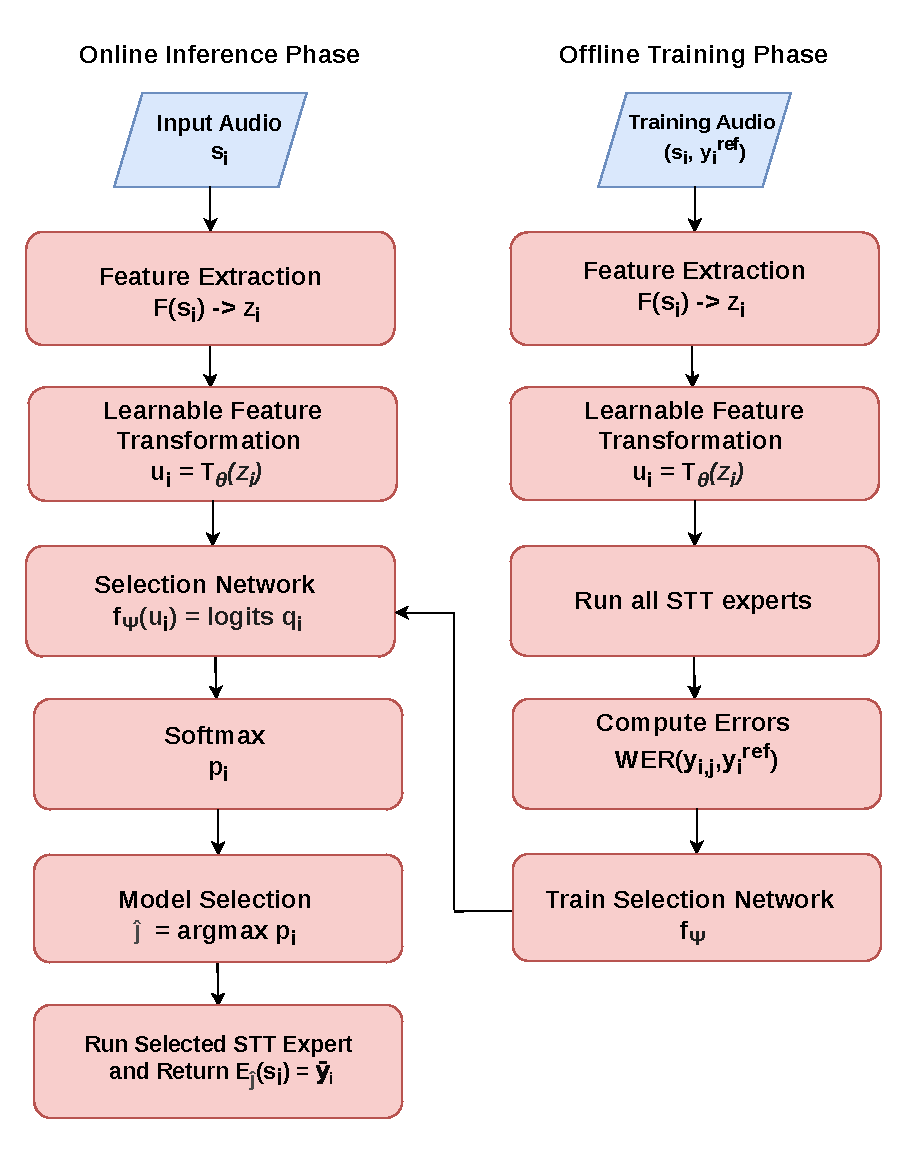
\includegraphics[width=1\linewidth]{figures/diagram.pdf}
        \caption{Overview of the FASTT framework. The offline phase extracts acoustic
        features, applies a learnable feature transformation, and trains the selection
        function using expected-WER minimization. At inference, only the selected
        STT expert is executed, introducing minimal overhead beyond a single
        model run.}
        \label{fig:feature-adaptive-diagram}
    \end{figure}

    \subsection{Algorithm Overview}

 The algorithm consists of two phases: an offline training phase and an
online inference phase, as illustrated in
Fig.~\ref{fig:feature-adaptive-diagram}. In the offline phase, the
system learns how to predict the relative suitability of different STT
experts based on input-dependent audio characteristics. For each
labeled training input $\mathbf{s}_i$, the framework extracts a feature vector
$\mathbf{z}_i$ using the feature pipeline described in
Section~\ref{sec:features}. This feature representation includes acoustic
statistics, prosodic descriptors, signal-level measures, and neural
speech embeddings aggregated at the utterance level. To improve selection reliability in high-dimensional feature spaces,
the framework learns a parametric feature transformation that maps the
original feature vector $\mathbf{z}_i$ into a task-aligned
representation as shown in Fig.~\ref{fig:feature-adaptive-diagram}. This transformation reshapes the feature space to
better capture the relationship between acoustic characteristics and
expert performance. The transformed features are then passed to a
selection function that produces a weight vector over the candidate
STT experts $\{E_1,\dots,E_L\}$. The parameters of the feature
transformation and the selection function are learned during the
offline phase using evaluations of all experts on labeled audio clips,
minimizing the cumulative transcription loss defined in
Section~\ref{sec:problem_formulation}.

In the online inference phase, given a new input audio $\mathbf{s}_i$, the
system first extracts the feature vector $\mathbf{z}_i$ as shown in Fig.~\ref{fig:feature-adaptive-diagram}. The trained
selection model then computes a weight vector $\mathbf{w}_n$ over the
candidate experts based on the transformed feature representation. A
single expert $E_{i_j}$ is selected according to the highest predicted
probability, and the final transcription $y_{i,E_i}$ is obtained by
executing only that expert. Because only one STT model is executed at
inference time, the framework introduces only minimal computational overhead beyond a single model run while still exploiting performance diversity across multiple pretrained experts. The complete online inference procedure is summarized in Algorithm~\ref{alg:fa-online-overview}, and the full pipeline is illustrated in Fig.~\ref{fig:feature-adaptive-diagram}. 

    \begin{algorithm}
        [t] \small
        \caption{\small Online STT Model Selection via FASTT }
        \label{alg:fa-online-overview}

        \textbf{Inputs:}
        \begin{itemize}
            \item Unlabeled input audio clip $\mathbf{s}_i$

            \item Set of audio feature extraction functions $\mathbb{F}(\cdot)$

            \item Trained FASTT selection pipeline $f_{\text{FASTT}}$

            \item STT expert pool $\mathcal{E}=\{E_{1},\dots,M_{L}\}$
        \end{itemize}

        \textbf{Outputs:}
        \begin{itemize}
            \item Final transcription $\widehat{y}_{i}$ for audio $s_{i}$
        \end{itemize}

        \textbf{Inference Steps:}
        \begin{algorithmic}
            [1] \State Extract utterance-level features:
            $\mathbf{z}_{i}\leftarrow \mathbb{F}(s_{i})$ \State Apply the trained FASTT
            pipeline to compute selection logits:
            $\mathbf{q}_{i}\leftarrow f_{\text{FASTT}}(\mathbf{z}_{i})$ \State Normalize
            $\mathbf{q}_{i}$ via softmax to obtain weights $\mathbf{p}_{i}$
            \State Select expert model:
            \[
                j_{i}\leftarrow \arg\max_{j \in \{1,\dots,K\}}p_{i,j}
            \]
            \State Return final transcription:
            $\hat{y}_{i}\leftarrow E_{\hat{j}}(s_{i})$
        \end{algorithmic}
    \end{algorithm}

    \subsection{Feature Representation}
    \label{sec:features}

    For each incoming audio input $\mathbf{s}_i$, we construct a compact feature vector
    $\mathbf{z}_{i}\in \mathbb{R}^{p}$ to encode acoustic and contextual information
    relevant to STT performance as shown in \cref{fig:feature-adaptive-diagram}.
    These features summarize signal quality, phonetic content, speaker
    characteristics, and temporal dynamics \cite{rabiner1993fundamentals,li2023emotionalasr}.

    \subsubsection{Spectral–Phonetic Features}
    We extract 13 Mel-frequency cepstral coefficients (MFCCs) together with their
    first- and second-order derivatives ($\Delta$ and $\Delta\Delta$)
    \cite{davis1980mfcc,furui1986deltas}. Lower-order coefficients represent the
    coarse spectral envelope, while higher-order terms encode finer phonetic
    detail. The inclusion of temporal derivatives provides robustness to coarticulation,
    prosodic variation, and speaker-specific articulation \cite{rabiner1993fundamentals}.

    \subsubsection{Prosodic Features}
    Prosodic features, including pitch statistics (mean, range) and silence ratios
    derived from voice activity detection (VAD), characterize speaking rhythm, stress,
    and expressiveness \cite{sohn1999vad}. Such features are particularly
    valuable for identifying conditions where transcription accuracy may degrade
    under expressive, emotional, or noisy speech \cite{li2023emotionalasr}.

    \subsubsection{Neural Speech Embeddings}
    High-level speech representations are extracted from pretrained self-supervised
    encoders such as Wav2Vec2 and HuBERT \cite{baevski2020wav2vec,hsu2021hubert}.
    These embeddings encapsulate rich information about phonetic identity, speaker
    traits, and semantic context, complementing conventional low-level features.
    Because they require only a single encoder forward pass without full
    decoding, they introduce negligible overhead relative to the STT inference itself.
    Specifically, the SSL encoder forward pass typically requires less than 50ms
    per utterance on modern GPU hardware, which is an order of magnitude smaller
    than the full ASR decoding time. For resource-constrained deployment scenarios,
    lighter embedding models or knowledge-distilled variants could be
    substituted without modifying the framework.

    \subsubsection{Signal and Temporal Features}
    Signal-level features including signal-to-noise ratio (SNR), zero-crossing rate
    (ZCR), and spectral entropy quantify acoustic clarity and spectral
    irregularity \cite{schuller2013computational,eyben2015opensmile}. Temporal features
    such as utterance duration, speech rate, and pause ratio measure fluency and
    pacing, both of which significantly impact STT robustness
    \cite{ko2015audio,tripathi2020ttransducer}. The resulting feature vector $\mathbf{z}
    _{i}$ thus integrates spectral, prosodic, neural, and temporal features into
    a unified contextual representation for each input. This vector serves as the
    conditioning signal for the supervised selection function.

    \begin{remark}
        Our framework is feature-agnostic: The proposed framework does not
        assume or require any specific feature family. The selection network operates
        on a generic feature vector and can incorporate any set of discriminative
        features such as acoustic, linguistic, prosodic, model-intrinsic, or domain-specific
        features that correlate with relative STT performance. If alternative
        features provide better separation between candidate algorithms for a
        given application, they can be substituted or augmented without modifying
        the training procedure, loss function, or selection mechanism.
    \end{remark}

    \subsection{Learnable Feature Transformation}
    \label{subsec:feature_transformation}

    The feature representation $\mathbf{z}_{i}\in \mathbb{R}^{p}$ described in \cref{sec:features}
    captures diverse acoustic and embedding-based properties of the input audio.
    While such descriptors provide informative signals for expert selection, their
    raw representation may not be optimally structured for predicting relative expert
    performance. In particular, high-dimensional feature spaces may contain correlated
    dimensions or redundant information that can make the selection model more difficult
    to train when labeled selection data is limited.

    Classical approaches to dimensionality reduction in such settings include filter-based
    methods (e.g., mutual information ranking, variance thresholding), wrapper-based
    strategies (e.g., sequential feature selection)~\cite{guyon2003introduction,kohavi1997wrappers}, and embedded methods that
    couple feature selection with model training~\cite{friedman2001}. However,
    filter methods disregard inter-feature dependencies and their interaction
    with the downstream objective, wrapper approaches have combinatorial search costs
    that scale poorly with $p$, and embedded methods are typically tied to
    specific model families. These limitations motivate a learnable, task-aligned
    feature transformation that can be jointly optimized with any downstream
    selector.

    We introduce a parametric mapping applied prior to the selection network
    that reshapes the geometry of the feature space without modifying the
    feature extraction pipeline itself, as illustrated in \cref{fig:feature-adaptive-diagram}.
    The transformed representation is defined as
    %
    \[
        \mathbf{u}_{i}= \mathbb{T}_{\theta}(\mathbf{z}_{i}),
    \]
    %
    where $\mathbb{T}_{\theta}: \mathbb{R}^{p}\rightarrow \mathbb{R}^{d'}$
    denotes a parametric transformation with learnable parameters $\theta$, and $\mathbf{u}
    _{i}$ serves as the input to the downstream expert selection function. The
    optimization strategy for $\theta$ depends on whether the downstream
    selector is differentiable, as discussed in \cref{subsec:selection_network}.
    We present several transformation variants below; all are compatible with any
    selector variant within the framework.

    \subsubsection{Diagonal Feature Gating}

    As a capacity-controlled transformation, we consider feature-wise scaling:
    %
\[
\mathbf{u}_i = \mathbf{q} \odot \mathbf{z}_i,
\]
    %
    where $\mathbf{q}\in \mathbb{R}^{p}$ is a learnable gating vector and
    $\odot$ denotes element-wise multiplication. Each component $q_{j}$ assigns an
    importance weight to the corresponding feature dimension $j$. This
    formulation acts as a differentiable feature-selection mechanism: dimensions
    with small $q_{j}$ values are effectively suppressed, while informative
    features receive larger weights. Because the number of additional parameters
    is limited to $d$, the diagonal gating transformation provides a simple yet
    effective mechanism for controlling overfitting in high-dimensional, data-limited
    regimes. To promote sparsity and stability, we apply combined $\ell_{1}$/$\ell
    _{2}$ regularization:
    %
    \[
        \lambda_{1}\|\mathbf{q}\|_{1}+ \lambda_{2}\|\mathbf{q}\|_{2}^{2}.
    \]
    %
    \subsubsection{Linear Feature Transformation}
    A more expressive alternative is a full linear projection:
    %
      \[
    \mathbf{u}_i = \mathbf{W}\mathbf{z}_i + \mathbf{b},
    \]
    %
    where $\mathbf{W}\in \mathbb{R}^{d' \times p}$ is a learnable projection matrix
    and $\mathbf{b}\in \mathbb{R}^{d'}$ is a bias vector. This transformation
    allows the model to reweight and mix the original feature dimensions in a
    task-aligned manner. By choosing $d' < p$, the transformation acts as a
    dimensionality-reduction mechanism. Weight decay regularization is applied to
    $\mathbf{W}$ to control overfitting.

    \subsubsection{Low-Rank Linear Transformation}

    While the full linear transformation allows arbitrary mixing of feature
    dimensions, it may introduce a large number of parameters when $p$ is high.
    To provide a more capacity-controlled alternative, we consider a low-rank factorization
    of the projection matrix:
    %
    \[
        \mathbf{u}_{i}= \mathbf{W}_{2}\mathbf{W}_{1}\mathbf{z}_{i},
    \]
    %
    where $\mathbf{W}_{1}\in \mathbb{R}^{r \times p}$, $\mathbf{W}_{2}\in \mathbb{R}
    ^{d' \times r}$, and $r \ll \min(p,d')$ is a bottleneck dimension. This factorization
    constrains the rank of the projection, allowing the model to capture
    interactions between feature dimensions while reducing the number of
    learnable parameters.

    \subsubsection{Nonlinear Feature Transformation}

    To capture nonlinear feature interactions that may affect relative expert performance,
    we consider a nonlinear bottleneck transformation:
    %
    \[
        \mathbf{u}_{i}= \mathbf{W}_{2}\, \sigma(\mathbf{W}_{1}\mathbf{z}_{i}),
    \]
    %
    where $\sigma(\cdot)$ is an element-wise activation function (e.g., ReLU or
    GELU), $\mathbf{W}_{1}\in \mathbb{R}^{r \times p}$ and
    $\mathbf{W}_{2}\in \mathbb{R}^{d' \times r}$ are learnable weight matrices, and
    $r \ll \min(p,d')$ is the bottleneck dimension. The bottleneck structure
    constrains the parameter count and helps prevent overfitting when labeled
    selection data is limited.

    \begin{remark}
        The proposed framework is flexible with respect to the choice of feature
        transformation. In addition to the variants presented here, other parametric
        transformations such as deeper neural encoders, kernel-based mappings, or
        representation learning modules could be used without modifying the overall
        pipeline. All transformation variants are evaluated in
        \cref{sec:experiments}.
    \end{remark}

    \subsection{Selection Objective}
    \label{subsec:selection_objective}

    Given the transformed feature vector $\mathbf{u}_{i}\in \mathbb{R}^{d'}$
    obtained from the feature transformation stage described in
    \cref{subsec:feature_transformation}, the goal of the selection function is to
    assign preference scores to a set of $L$ pretrained STT experts $\mathcal{E}=
    \{E_{1},\dots,E_{L}\}$. We define the selection function as a parametric
    mapping
    %
    \[
        f_{\psi}(\mathbf{u}_{i}) = \mathbf{q}_{i}\in \mathbb{R}^{L},
    \]
    %
    where $\psi$ denotes the trainable parameters and
    $\mathbf{q}_{i}= (q_{i,1}, \dots,q_{i,L})$ represents the logits associated
    with the candidate STT experts. Each component $q_{i,j}$ reflects the relative
    suitability of expert $E_{j}$ for the audio input $\mathbf{s_{j}}$. We apply a 
    softmax operation to the logits to obtain a normalized selection probability
    for each expert model:
    \begin{equation}
        p_{i,j}= \frac{\exp(q_{i,j})}{\sum_{m=1}^{L}\exp(q_{i,m})}, \qquad j=1,\dots
        ,L, \label{eq:softmax_router}
    \end{equation}
    where $p_{i,j}$ denotes the probability assigned to expert $E_{j}$. Given
    these probabilities, we define the expected transcription loss for the audio
    clip $s_{i}$ as
    \begin{equation}
        \mathcal{L}_{n}= \sum_{j=1}^{L}p_{i,j}\,\mathrm{WER}(y_{i,j},\,y_i^{\mathrm{ref}}), \label{eq:expected_loss}
    \end{equation}
    where $\,y_i^{\mathrm{ref}}$ is the reference transcription. The WER between a hypothesis
    transcription $y_{i,j}$ and the reference $\,y_i^{\mathrm{ref}}$ is defined as
    $\mathrm{WER}(y_{i,j}, \,y_i^{\mathrm{ref}}) = \frac{S + I + D}{|\,y_i^{\mathrm{ref}}|}$, where $S$, $I$, and
    $D$ denote the numbers of substitutions, insertions, and deletions obtained from
    a standard Levenshtein alignment~\cite{li2014overviewrobust}.

    \begin{remark}
        Although we use WER as the optimization objective due to its widespread use
        and interpretability in speech recognition research~\cite{yu2016asrdeep,li2014overviewrobust},
        other transcription quality metrics such as CER or task-specific error
        measures could also be used within the same framework.
    \end{remark}

    The overall training objective minimizes the expected transcription error
    across the dataset:
    \begin{equation}
        \min_{\theta,\psi}\mathcal{L}= \frac{1}{N}\sum_{n=1}^{N}\mathcal{L}_{n}=
        \frac{1}{N}\sum_{n=1}^{N}\sum_{j=1}^{L}p_{i,j}\,\mathrm{WER}(y_{i,j},\,y_i^{\mathrm{ref}}
        ). \label{eq:training_objective}
    \end{equation}

    During training, the WER values $\mathrm{WER}(y_{i,j},\,y_i^{\mathrm{ref}})$ are treated as
    fixed constants obtained from offline evaluation of the STT experts. The
    optimization strategy for the feature transformation parameters~$\theta$ and
    the selection function parameters~$\psi$ depends on whether the selection
    function is differentiable with respect to its inputs and parameters, as discussed
    in the following subsection.

    \subsection{Joint Feature and Model Selection}
    \label{subsec:selection_network}

    A key contribution of the FASTT framework is the joint
    training of the feature transformation $\mathbb{T}_{\theta}$ and the selection
    function $f_{\psi}$. Instead of performing feature selection and model
    selection as two separate steps, FASTT learns both components together
    using the expected transcription error. This joint training aligns
    the feature representation with the model selection task. 
    
    The framework supports two optimization paths depending on the differentiability
    of the selection function.

    \subsubsection{FASTT for Differentiable Model Selectors}
    \label{subsubsec:diff_selectors}

    When the selection function $f_{\psi}(\cdot)$ is differentiable with respect
    to its parameters $\psi$ and its inputs $\mathbf{u}_{i}$, the parameters
    $\theta$ and $\psi$ are optimized jointly using standard backpropagation.
    Gradients of the expected word error rate (WER) objective flow from the softmax probabilities,
    through the selection network, and into the feature transformation. This strategy enables
    end-to-end feature adaptation in a single training loop without requiring any auxiliary steps.

    As a representative differentiable model, we use Soft Decision Trees (SDTs). SDTs are hierarchical models where each internal node makes a soft, probabilistic routing decision based on a linear combination of features. Because these routing decisions are continuous rather than completely discrete, SDTs are fully differentiable and suitable for gradient descent. We construct our selector, FASTT-SDT, using an additive ensemble of SDTs, as in \cite{karaca2026soft}. The model consists
    of $B$ sequential boosting rounds. At each round $b$, a per-round feature transformation
    $\mathbb{T}_{\theta_b}(\cdot)$ is applied to the input features, followed by
    a soft decision tree $h_{b}(\cdot)$ providing $L$ logits. The final output is the sum of logits
    across all boosting rounds:
    \begin{equation}
        \mathbf{q}_{i}= \sum_{b=1}^{B}h_{b}\!\left(\mathbb{T}_{\theta_b}(\mathbf{z}
        _{i})\right). \label{eq:bfs_output}
    \end{equation}

    At each round, the current tree is fit on the gradient of the previous predictions. The per-round feature transformation $\mathbb{T}_{\theta_b}$ and the soft decision tree $h_{b}$ are optimized jointly using backpropagation on the expected-WER objective from \eqref{eq:training_objective}. 
    A key property of BFS is that each boosting round learns its
    own feature transformation, allowing different rounds to focus
    on different subsets or combinations of the input features.
    % When the diagonal gating transform is used, the gating vector
    % in $\mathbb{T}_{\theta_b}$ directly controls which features each round attends
    % to, providing an interpretable and sparse feature selection
    % mechanism. When soft decision trees are used as the base
    % model $h_{b}$, each internal node performs a soft routing decision
    % using learned feature weights. The combination of per-round
    % gating and soft routing provides explicit, interpretable feature
    % importance through the magnitudes of the learned weights.
    The complete offline training procedure is given in Algorithm \ref{alg:fasttsdt_training}.
    \begin{algorithm}
        [t] \small
        \caption{Offline Training: FASTT for Differentiable Selectors}
        \label{alg:fasttsdt_training}

        \textbf{Inputs:}
        \begin{itemize}
            \item $\{(s_{1},\,y_1^{\mathrm{ref}}),\dots,(s_{N},\,y_N^{\mathrm{ref}})\}$: Labeled audio clips
                with reference transcriptions

            \item $\mathbb{F}$: Feature extraction pipeline

            \item $\mathcal{E}=\{E_{1},\dots,E_{L}\}$: Pretrained STT expert
                pool

            \item $B$: Number of boosting rounds
        \end{itemize}

        \textbf{Output:} Trained FASTT model $\{(\mathbb{T}_{\theta_b}, h_{b})\}_{b=1}^{B}$

        \begin{algorithmic}[1]
            \setcounter{ALG@line}{-1}
            \State \textbf{Offline data preparation:} \For{$n \gets 1$ \textbf{to} $N$}
            \State Extract features: $\mathbf{z}_{i}\gets \mathbb{F}(s_{i})$
            \For{each expert $E_{j}\in \mathcal{E}$} \State Transcribe:
            $y_{i,j}\gets E_{j}(s_{i})$ \State Compute: $\mathrm{WER}_{i,j}\gets
            \mathrm{WER}(y_{i,j},\,y_i^{\mathrm{ref}})$ \EndFor \EndFor \State Initialize ensemble
            prediction: $\hat{\mathbf{q}}^{(0)}_{i}\gets \mathbf{0}$ for all $i$
            \State \textbf{Boosted training:} \For{round $b \gets 1$ \textbf{to} $B$}
            \State Compute residual targets from $\hat{\mathbf{q}}^{(b-1)}_{i}$
            using \eqref{eq:expected_loss} \State Initialize per-round feature transform
            $\mathbb{T}_{\theta_b}$ \State Fit base model $h_{b}$ on $\{(\mathbb{T}
            _{\theta_b}(\mathbf{z}_{i}), \text{residual}_{i})\}$ \State Jointly optimize
            $\theta_{b}$ and $h_{b}$ via backpropagation with $\ell_{1}$ regularization
            on $\theta_{b}$ \State Update ensemble:
            $\hat{\mathbf{q}}^{(b)}_{i}\gets \hat{\mathbf{q}}^{(b-1)}_{i}+ h_{b}(\mathbb{T}_{\theta_b}(\mathbf{z}_{i}))$
            \EndFor \State \textbf{Online inference:} For new audio $s_{i}$,
            compute
            $\mathbf{q}_{i}= \sum_{b=1}^{B}h_{b}(\mathbb{T}_{\theta_b}(\mathbb{F}(s_{i})))$, apply softmax, select $\hat{j}= \arg\max_{j}p_{i,j}$
        \end{algorithmic}
    \end{algorithm}

    \subsubsection{FASTT for Non-Differentiable Model Selectors}
    \label{subsubsec:nondiff_selectors}

    Tree-based ensemble methods such as gradient-boosted decision trees perform
    well on structured tabular data and provide strong regularization.
    However, they are not differentiable with respect to their input features. Gradients cannot be propagated through the discrete tree structure to update the parameters of the feature transformation $\mathbb{T}_{\theta}$. This creates an optimization challenge since $\theta$ and $\psi$ cannot be trained jointly via standard backpropagation.

    To enable joint adaptation without requiring differentiability, FASTT uses an alternating optimization strategy \cite{bertsekas1999nonlinear}. We decompose the joint training problem into two subproblems that are optimized iteratively:
    
    \begin{enumerate}
        \item \emph{Selector update (fix $\theta$, optimize $\psi$):} Given the
            current feature transformation $\mathbb{T}_{\theta}$, compute the transformed
            features $\mathbf{u}_{i}= \mathbb{T}_{\theta}(\mathbf{z}_{i})$ and train
            the tree-based selector on these features.
            
        \item \emph{Transform update (fix $\psi$, optimize $\theta$):} With the
            tree structure strictly fixed, update the feature transformation parameters $\theta$. 
            % Because backpropagation through the tree is invalid, $\theta$ may be updated either by relying on a continuous, differentiable surrogate approximation of the selector (e.g., using straight-through estimators or localized gradient approximations), or through derivative-free search methods. In practice, depending on the computational budget, this transform update step may be simplified or omitted.
    \end{enumerate}

    This alternating procedure is repeated for a fixed number of iterations. The complete training procedure is given in Algorithm \ref{alg:nondiff_training}.

    As a representative non-differentiable selector in this path, we utilize XGBoost \cite{chen2016xgboost}. Crucially, the selector must minimize the expected-WER objective instead of conventional classification or regression losses. Standard objectives like cross-entropy typically align with categorical targets, whereas FASTT requires minimizing a continuous, sequence-level transcription error (WER) over a probability distribution of distinct STT domains. Therefore, XGBoost is trained with a \emph{custom objective function}. We supply the algorithm with specifically formulated first- and second-order derivatives to seamlessly integrate expected-WER minimization into the tree-building process.
    
    Let $g_{i,j}$ and $h_{i,j}$ denote the first- and second-order derivatives of $\mathcal{L}_{i}$ with respect to the output logit $q_{i,j}$:
    \begin{align}
        g_{i,j} & = \frac{\partial \mathcal{L}_{i}}{\partial q_{i,j}} = p_{i,j}\left(\mathrm{WER}(y_{i,j}, \,y_i^{\mathrm{ref}})-\mathcal{L}_{i}\right). \label{eq:gradient}
    \end{align}
    To reduce computational cost and maintain stable split gains, we use a diagonal approximation to the Hessian:
    \begin{align}
        h_{i,j} & = \frac{\partial^{2}\mathcal{L}_{i}}{\partial q_{i,j}^{2}} = p_{i,j}(1-2p_{i,j}) \left(\mathrm{WER}(y_{i,j},\,y_i^{\mathrm{ref}})-\mathcal{L}_{i}\right). \label{eq:hessian}
    \end{align}
    We clip negative Hessian values to a small positive constant to ensure stable tree building \cite{chen2016xgboost}. 

    \begin{algorithm}
        [t] \small
        \caption{Offline Training: FASTT for Non-Differentiable Selectors}
        \label{alg:nondiff_training}

        \textbf{Inputs:}
        \begin{itemize}
            \item $\{(s_{1}, \,y_1^{\mathrm{ref}}), \ldots, (s_{N}, \,y_N^{\mathrm{ref}})\}$: Labeled audio
                clips with reference transcriptions

            \item $\mathbb{F}$: Feature extraction pipeline

            \item $\mathcal{E}= \{E_{1}, \ldots, E_{K}\}$: Pretrained STT expert
                pool

            \item $\mathbb{T}_{\theta}$: Learnable feature transformation

            \item $T$: Number of alternating iterations
        \end{itemize}

        \textbf{Output:} Trained feature transformation $\mathbb{T}_{\theta}$ and selector $f_{\psi}$

        \begin{algorithmic}[1]
            \setcounter{ALG@line}{-1}
            \State \textbf{Offline data preparation:} \For{$i \gets 1$ \textbf{to} $N$}
            \State Extract features: $\mathbf{z}_{i}\gets \mathbb{F}(s_{i})$
            \For{each expert $E_{j}\in \mathcal{E}$} \State Transcribe:
            $y_{i,j}\gets E_{j}(s_{i})$ \State Compute: $\mathrm{WER}_{i,j}\gets
            \mathrm{WER}(y_{i,j}, \,y_i^{\mathrm{ref}})$ \EndFor \EndFor \State \textbf{Alternating
            optimization:} \For{iteration $t = 1,\ldots,T$} \State Transform features:
            $\mathbf{u}_{i}\gets \mathbb{T}_{\theta}(\mathbf{z}_{i})$ for all
            $i$ \State Compute softmax weights $\mathbf{p}_{i}$ via \eqref{eq:softmax_router}
            \State Compute per-instance gradients $g_{i,j}$ and Hessians $h_{i,j}$
            via \eqref{eq:gradient}--\eqref{eq:hessian} \State \textbf{Selector
            update:} Train XGBoost $f_{\psi}$ on $\{\mathbf{u}_{i}\}$ using the custom
            WER-based targets \State Obtain updated logits:
            $\mathbf{q}_{i}\gets f_{\psi}(\mathbf{u}_{i})$ \State \textbf{Transform
            update:} Fix $f_{\psi}$; optimize $\theta$ using a valid surrogate gradient or continuous approximation \EndFor \State \textbf{Online
            inference:} For new audio $s_{i}$, compute
            $\mathbf{q}_{i}= f_{\psi}(\mathbb{T}_{\theta}(\mathbb{F}(s_{i})))$, apply
            softmax, select $\hat{j}= \arg\max_{j}p_{i,j}$
        \end{algorithmic}
    \end{algorithm}

    \begin{remark}
        The framework is flexible and can accommodate a wide range of learning algorithms
        for the selection function. In addition to the variants presented here, other
        architectures such as transformers~\cite{vaswani2017attention} or alternative
        supervised learning algorithms could be used without modifying the overall
        pipeline.
    \end{remark}

    \subsection{Sampling Strategy}
    \label{subsec:sampling}

    Given the selection probabilities $\mathbf{p}_{i}= (p_{i,1},\dots,p_{i,K})$
    produced by the selection function, we choose the final expert as
    \[
        \hat{j}= \arg\max_{j \in \{1,\dots,L\}}p_{i,j}.
    \]
    The selected expert is then executed to produce the final transcription $\hat
    {y}_{i}= E_{\hat{j}}(s_{i})$ as shown in \cref{fig:feature-adaptive-diagram}.
    Because only a single STT expert is executed, the computational cost of inference
    remains comparable to that of a single-model system. The selection function
    itself introduces negligible overhead since it operates on pre-extracted
    features and involves only lightweight computation relative to the STT
    models.
    
    \section{Mathematical Proof of Convergence}
    \label{subsec:theoretic}

    We provide convergence guarantees for the selector optimization procedures
    presented in~\cref{subsec:selection_network}. Specifically, we show that
    under mild regularity conditions, both training procedures converge to a first-order
    stationary point of the training objective.

    The proofs hold for any smooth loss with bounded curvature, consistent with the framework's loss-agnostic design. Our convergence analysis focuses on the
    optimization of the selector parameters for a fixed feature transformation. In
    the full framework, the transformation parameters are updated either jointly
    (for differentiable selectors) or through alternating optimization (for tree-based
    selectors), which preserves the stationary-point guarantees for the selector
    subproblem. The same convergence guarantees apply to alternative admissible
    objectives (e.g., cross-entropy, MSE, or other smooth sequence-level surrogates)
    that satisfy the smoothness assumptions used in the analysis.
    
    \vspace{-0.30em}
    
    \subsection{XGBoost-based Selector}
    
    For the XGBoost-based selector, we prove convergence under our custom WER-based objective by extending standard second-order boosting theory. Assuming bounded loss values, Lipschitz-continuous gradients, and a weak-learner edge condition, we obtain a monotone descent property. Let \(L(\mathbf{q^{(n)}})\) denote the training loss evaluated at the current logits \(\mathbf{q^{(n)}}\). 
    
    Under these assumptions, and for a sufficiently small step size \(\eta\), the training dynamics admit the following descent inequality:
    \begin{equation}
        L_{n+1} \leq L_n - \gamma \| \nabla L(\mathbf{q^{(n)}}) \|^2,
    \end{equation}
    where \(\gamma > 0\) is a constant that depends on the learning rate, the weak-learner edge, and the smoothness of the loss function. Summing over iterations yields an \(\mathcal{O}(1/N)\) convergence rate to a first-order stationary point. Full derivations and the explicit form of \(\gamma\) are provided in Appendix~\ref{appendix:convergence}.
    
    
    \subsection{Neural Selector (MLP / FASTT-SDT)}
    
    For the neural selector, we rely on standard non-convex optimization results under smoothness of the loss function and bounded variance of the stochastic gradients. Under these assumptions, the training dynamics satisfy:
    \begin{itemize}
        \item an $\mathcal{O}(1/N)$ convergence rate for full-batch gradient descent, and
        \item an $\mathcal{O}(1/\sqrt{N})$ convergence rate for mini-batch SGD,
    \end{itemize}
    implying convergence to a first-order stationary point. Detailed derivations are provided in Appendix~\ref{appendix:convergence}.

        \begin{remark}
        These results characterize the convergence behavior of the \emph{selector
        optimization} under fixed or jointly updated feature transformations. Formal
        convergence guarantees for the end-to-end joint system (feature
        transform + selector) in the non-differentiable alternating optimization
        case remain an open question and are left for future investigation.
    \end{remark}

    \section{Experiments and Results}
    \label{sec:experiments}

    We evaluate the proposed FASTT framework by using the selector and transformation
    variants described in \cref{subsec:selection_network,subsec:feature_transformation}.
    The experiments are designed to (i)~compare the framework variants against
    external baselines and classical feature selection strategies, (ii)~ablate the
    contribution of different feature transformation and selector choices, and (iii)~analyze
    computational overhead.

    \subsection{Datasets and Feature Extraction}
    \label{subsec:datasets_features}

    We construct a heterogeneous evaluation corpus by aggregating clips from four
    publicly available English speech datasets that span a wide range of acoustic
    conditions. The corpus includes LibriSpeech~\cite{panayotov2015librispeech}
    (read audiobook speech from \textit{test-clean} and \textit{test-other} splits),
    Common Voice~\cite{ardila2020commonvoice} (crowd-sourced recordings with
    diverse speaker demographics and recording equipment), VoxPopuli's English accented subset ~\cite{wang2021voxpopuli}
    (European Parliament speech with accented English and varying room acoustics),
    and challenging SDM subset of AMI~\cite{carletta2005ami} (meeting recordings using both single distant microphones). This corpus is designed so that no single STT model dominates across all conditions, providing a meaningful testbed for adaptive model selection. The dataset statistics are summarized in Table~\ref{tab:dataset_stats}.

    \begin{table}[t]
    \centering
    \caption{Dataset statistics.}
    \label{tab:dataset_stats} \small
    \begin{tabular}{lcccc}
        \toprule \textbf{Dataset} & Ami (SDM)  & Libri & CV   & VoxP.\\
        \midrule Total Clips      & 4091 & 10500 & 8200 & 6400  \\
        Features                  & 1672 & 1672  & 1672 & 1672  \\
        Train Size                & 3272 & 8400  & 6560 & 5120  \\
        Test Size                 & 819  & 2100  & 1640 & 1280  \\
        \bottomrule
    \end{tabular}
\end{table}

    Each clip is represented by a $p\!=\!1672$-dimensional feature vector $\mathbf{z}
    _{i}$ composed of the feature groups described in \cref{sec:features}.
    Specifically, the vector concatenates 78 spectral--phonetic features (MFCCs with
    $\Delta$/$\Delta\Delta$), 17 prosodic and VAD features, 14 channel and noise
    features, 8 signal complexity features, 1536 neural embeddings (mean-pooled Wav2Vec2
    and HuBERT embeddings, 768 dimensions each), and 19 embedding statistics and
    metadata features. This high-dimensional representation motivates the learnable
    feature transformation: directly training a selector on all 1672 features in
    data-scarce regimes can lead to overfitting and unstable selection.

    \subsection{Models and Baselines}
    \label{subsec:models_baselines}

    \subsubsection{Individual STT Experts}
    We employ $L\!=\!3$ pretrained STT models as the expert pool $\mathcal{E}$:
    Whisper-large-v3~\cite{radford2022whisper} (a transformer encoder--decoder
    trained on 680k hours of weakly supervised web audio), Parakeet-TDT-0.6b-v2 (a
    FastConformer--Transducer model optimized for English ASR with token-and-duration
    transducer decoding), and Canary-Qwen-2.5b (a multi-task encoder--decoder
    combining a FastConformer audio encoder with a Qwen-2.5 language model
    backbone). For each audio clip~$s_{i}$, all three models are run offline to obtain
    transcriptions $\{y_{i,j}\}_{j=1}^{3}$ and their associated word error rates
    against reference transcripts.

    \subsubsection{External Baselines}
    We compare against non-learned and simple baselines that do not use the FASTT
    feature transformation pipeline: (i)~ROVER~\cite{fiscus1997rover}, which aligns
    hypotheses from all $K$ models via pivot-based word alignment and applies majority
    voting; (ii)~Random Ensemble, which selects a model uniformly at random for each
    utterance. We additionally report the Oracle (per-clip selection of the best
    model) as an upper bound on selection performance.

    \subsubsection{Classical Feature Selection Strategies}
    To demonstrate the advantage of learned, task-aligned feature transformations
    over classical approaches, we evaluate four classical feature selection
    baselines. These methods apply feature selection as a fixed preprocessing step,
    followed by training a selector on the reduced feature set:
    \begin{itemize}
        \item SelectKBest-MLP: The top $k$ features are selected using
            univariate statistical tests (ANOVA F-value), and an MLP is trained on
            the selected features.

        \item SelectKBest-XGBoost: Same feature selection, followed by an XGBoost
            selector.

        \item Wrapper-MLP: Sequential forward selection is used to greedily
            select a feature subset, with an MLP trained on the result.

        \item Wrapper-XGBoost: Same wrapper-based selection, followed by an XGBoost
            selector.
    \end{itemize}
    All classical methods use the same expected-WER objective, ensuring a fair
    comparison with the FASTT framework.

    \subsubsection{FASTT Variants}
    We evaluate two representative variants within the FASTT framework, corresponding
    to the differentiable and non-differentiable optimization paths described in~\cref{subsec:selection_network}:
    \begin{itemize}
        \item FASTT-SDT (differentiable path): The Boosted Feature-adaptive
            Selector with soft decision trees as the base model and diagonal
            feature gating, trained end-to-end with per-round feature adaptation
            and $\ell_{1}$-penalized routing.

        \item FASTT-XGBoost (non-differentiable path): An XGBoost-based selector
            with learned diagonal feature gating, trained via the alternating optimization
            procedure described in~\cref{subsubsec:nondiff_selectors}.
    \end{itemize}
    The choice of base model and selector within each path is further studied in
    the ablation experiments.

    \subsection{Training Setup and Evaluation}
    \label{subsec:training_setup}

    The dataset is split into 80\% training and 20\% test sets, stratified by
    source dataset where possible. Within the training portion, 15\% is further reserved
    for validation to facilitate early stopping and hyperparameter selection. To
    ensure a fair comparison, all learned methods receive an equal computational
    budget for hyperparameter tuning. We employ Optuna~\cite{akiba2019optuna}
    with a Tree-structured Parzen Estimator (TPE) sampler. The hyperparameter search
    spaces are given in Table~\ref{tab:hp_spaces}. The primary evaluation metric
    is the \emph{mean WER of the selected model} across all test clips:
    \begin{equation}
        \text{WER}_{\text{method}}= \frac{1}{|\mathcal{D}_{\text{test}}|}\sum_{n
        \in \mathcal{D}_{\text{test}}}\ell\!\left(y_{i,\, j_i},\, \,y_i^{\mathrm{ref}}\right),
    \end{equation}
    where $j_{i}$ is the model index selected by the evaluating method.

    \begin{table}[t]
    \centering
    \caption{Hyperparameter search spaces. 
    % XGBoost spaces are shared across all XGBoost-based methods (raw features, SelectKBest, Wrapper, and FASTT-XGBoost).
    }
    \label{tab:hp_spaces} \small
    \begin{tabular}{@{}lll@{}}
        \toprule \textbf{Method}                                               & \textbf{Parameter}  & \textbf{Search space}      \\
        \midrule \multicolumn{3}{l}{\textit{Model selector hyperparameters}}    \\
        \midrule \multirow{7}{*}{XGBoost}                                      & Num estimators      & \{100, 500, 1000\}         \\
                                                                               & Learning rate       & \{1e-2, 2e-2, 5e-2, 1e-1\} \\
                                                                               & Max depth           & \{4, 6, 8, 10\}            \\
                                                                               & Subsample           & \{0.6, 0.8, 1.0\}          \\
                                                                               & Column subsample    & \{0.5, 0.8, 1.0\}          \\
                                                                               & Min child weight    & \{1, 4, 10\}               \\
                                                                               & Reg lambda          & \{0.1, 1.0, 10.0\}         \\
        \midrule \multirow{4}{*}{MLP}                                          & Learning rate       & \{1e-4, 5e-4, 1e-3\}       \\
                                                                               & Weight decay        & \{1e-5, 1e-4, 1e-3\}       \\
                                                                               & Batch size          & \{512, 1024, 2048\}        \\
                                                                               & Dropout rate        & \{0.1, 0.2, 0.3\}          \\
        \midrule \multirow{4}{*}{Soft Decision Tree}                           & Trees per layer     & \{10, 50, 100\}            \\
                                                                               & Tree depth          & \{3, 4, 5\}                \\
                                                                               & Lambda ($\ell_{1}$) & \{0.01, 0.1, 1.0\}         \\
                                                                               & Temperature         & \{0.5, 1.0, 2.0\}          \\
        \midrule \multicolumn{3}{l}{\textit{Feature selection hyperparameters}} \\
        \midrule SelectKBest                                                   & $k$ (num. features) & \{50, 100, 200, 500\}      \\
        \midrule Wrapper                                                       & Max features        & \{50, 100, 200\}           \\
        % \midrule \multicolumn{3}{l}{\textit{Framework-level hyperparameters (FASTT variants)}} \\
        \midrule \multirow{4}{*}{FASTT}                                        & Boosting rounds     & \{2, 3, 5\}                \\
                                                                               & Learning rate       & \{1e-4, 5e-4, 1e-3\}       \\
                                                                               & Weight decay        & \{1e-05, 1e-4, 1e-3\}      \\
                                                                               & Iterations          & \{3, 5, 10\}               \\
        \bottomrule
    \end{tabular}
\end{table}

    \subsection{Results and Discussion}
    \label{subsec:results_discussion}

    \subsubsection{Transcription Performance}

    Table~\ref{tab:wer_results} presents the overall and per-dataset WER evaluated
    on the held-out test set.
    % For completeness, cross-validation training WERs are also reported in Table~\ref{tab:cv_train_wer}, verifying that the proposed approach does not suffer from substantial overfitting.
    Several observations emerge from the performance analysis. First, all FASTT
    framework variants consistently outperform both external baselines and
    classical feature selection strategies, confirming that the combination of learned
    feature transformation and task-aligned selection yields a systematic advantage
    over fixed-preprocessing approaches. Second, the FASTT variants achieve the best
    overall performance, outperforming the competitor model selector baselines
    across all datasets, under high dimensionality conditions. This demonstrates
    the effectiveness of the integrated feature selection within the FASTT
    architecture. Third, the classical feature selection baselines (SelectKBest,
    Wrapper) improve over raw-feature selectors but fall short of the FASTT variants,
    validating the importance of joint optimization. Performance differences between
    methods are most pronounced on acoustically challenging datasets such as AMI
    and VoxPopuli, where the benefit of adaptive selection is maximized. Conversely,
    on cleaner datasets like LibriSpeech, all methods closely approach the oracle
    performance.

    \begin{table}[t]
    \centering
    \caption{Test WER across datasets.}
    \label{tab:wer_results} \small
    \begin{tabular}{lcccc}
        \toprule \textbf{Method}                                         & Ami             & Libri.          & CV              & VoxP.           \\
        \midrule \multicolumn{5}{l}{\textit{Individual STT Models}}       \\
        Whisper-large-v3                                                 & 0.3105          & 0.0485          & 0.0725          & 0.2150          \\
        Parakeet-TDT-0.6b                                                & 0.2995          & 0.0435          & 0.0730          & 0.1985          \\
        Canary-Qwen-2.5b                                                 & 0.2530          & 0.0412          & 0.0614          & 0.2130          \\
        \midrule \multicolumn{5}{l}{\textit{External Baselines}}          \\
        Random Ensemble                                                  & 0.2810          & 0.0440          & 0.0675          & 0.2090          \\
        ROVER                                                            & 0.2910          & 0.0415          & 0.0640          & 0.1910          \\
        \midrule \multicolumn{5}{l}{\textit{Classical Feature Selection}} \\
        SelectKBest-SDT                                                  & 0.2710          & 0.0420          & 0.0630          & 0.1890          \\
        SelectKBest-XGBoost                                              & 0.2690          & 0.0422          & 0.0625          & 0.1892          \\
        Wrapper-SDT                                                      & 0.2660          & 0.0418          & 0.0618          & 0.1885          \\
        Wrapper-XGBoost                                                  & 0.2640          & 0.0419          & 0.0616          & 0.1886          \\
        \midrule \multicolumn{5}{l}{\textit{FASTT Framework Variants}}    \\
        FASTT-XGBoost                                                    & 0.2507          & \textbf{0.0407} & 0.0572          & 0.1805          \\
        FASTT-SDT                                                        & \textbf{0.2505} & 0.0413          & \textbf{0.0565} & \textbf{0.1801} \\
        \midrule Oracle                                                  & \textit{0.1491} & \textit{0.0247} & \textit{0.0361} & \textit{0.1387} \\
        \bottomrule
    \end{tabular}
\end{table}
    % \begin{table}[t]
    \centering
    \caption{Training WER (cross-validation) across datasets.}
    \label{tab:cv_train_wer} \small
    \begin{tabular}{lcccc}
        \toprule \textbf{Method}                                         & Ami             & Libri.          & CV              & VoxP.           \\
        \midrule \multicolumn{5}{l}{\textit{Individual STT Models}}       \\
        Whisper-large-v3                                                 & 0.4061          & 0.0440          & 0.1200          & 0.1800          \\
        Parakeet-TDT-0.6b                                                & 0.3230          & 0.0510          & 0.1080          & 0.1600          \\
        Canary-Qwen-2.5b                                                 & 0.2906          & 0.0460          & 0.1100          & 0.1400          \\
        \midrule \multicolumn{5}{l}{\textit{External Baselines}}          \\
        Random Ensemble                                                  & 0.3391          & 0.0470          & 0.1127          & 0.1600          \\
        ROVER                                                            & 0.2800          & 0.0390          & 0.0980          & 0.1320          \\
        \midrule \multicolumn{5}{l}{\textit{Classical Feature Selection}} \\
        SelectKBest-SDT                                                  & 0.2680          & 0.0370          & 0.0910          & 0.1260          \\
        SelectKBest-XGBoost                                              & 0.2660          & 0.0365          & 0.0900          & 0.1250          \\
        Wrapper-SDT                                                      & 0.2630          & 0.0355          & 0.0890          & 0.1240          \\
        Wrapper-XGBoost                                                  & 0.2610          & 0.0350          & 0.0880          & 0.1220          \\
        \midrule \multicolumn{5}{l}{\textit{FASTT Framework Variants}}    \\
        FASTT-XGBoost                                                    & 0.2520          & 0.0325          & 0.0860          & 0.1180          \\
        \textbf{FASTT-SDT}                                               & \textbf{0.2450} & \textbf{0.0310} & \textbf{0.0830} & \textbf{0.1130} \\
        \midrule Oracle                                                  & \textit{0.2300} & \textit{0.0280} & \textit{0.0750} & \textit{0.1050} \\
        \bottomrule
    \end{tabular}
\end{table}
    % \begin{table}[t]
\centering
\caption{Cross-Validation Validation WER comparison across datasets.}
\label{tab:cv_val_wer}
\small
\begin{tabular}{lcccc}
\toprule
\textbf{Model} & Ami & Libri. & CV & VoxP. \\
\midrule
Whisper-large-v3 & 0.4851 & 0.0460 & 0.1280 & 0.1900 \\
Parakeet-TDT-0.6b & 0.3362 & 0.0530 & 0.1120 & 0.1680 \\
Canary-Qwen-2.5b & 0.3648 & 0.0490 & 0.1180 & 0.1450 \\
Random Ensemble & 0.3985 & 0.0493 & 0.1193 & 0.1677 \\
ROVER & 0.3000 & 0.0410 & 0.1020 & 0.1380 \\
MLP & 0.3491 & 0.0440 & 0.1080 & 0.1430 \\
XGBoost & 0.3364 & 0.0430 & 0.1050 & 0.1410 \\
FASTT-BFS & \textbf{0.2950} & \textbf{0.0390} & \textbf{0.0980} & \textbf{0.1330} \\
Oracle & \textit{0.2700} & \textit{0.0360} & \textit{0.0880} & \textit{0.1230} \\
\bottomrule
\end{tabular}
\end{table}


    \subsubsection{Computational Complexity}
    To evaluate the efficiency of the proposed selection mechanism, we measure the
    selector training and inference times separately from STT decoding and feature
    extraction, as reported in Tables~\ref{tab:cv_fit_time} and~\ref{tab:cv_score_time}.
    We emphasize that these measurements reflect only the selector overhead; STT
    decoding and SSL feature extraction are performed offline and are common to
    all methods. Because FASTT executes only a single, dynamically chosen STT
    model during inference, the actual transcription time per utterance strictly
    matches that of running an individual model. In contrast, ROVER imposes a substantial
    multiplicative cost by requiring execution of all $L$ experts prior to alignment
    and voting.

    \begin{table}[t]
    \centering
    \caption{Selector training time (seconds) across datasets. STT decoding and feature
    extraction are performed offline and excluded from these measurements.}
    \label{tab:cv_fit_time} \small
    \begin{tabular}{lcccc}
        \toprule \textbf{Method}                                         & Ami     & Libri.  & CV      & VoxP.  \\
        \midrule \multicolumn{5}{l}{\textit{External Baselines}}          \\
        Random Ensemble                                                  & ---     & ---     & ---     & ---     \\
        ROVER                                                            & ---     & ---     & ---     & ---     \\
        \midrule \multicolumn{5}{l}{\textit{Classical Feature Selection}} \\
        SelectKBest-SDT                                                  & 2.15  & 8.40  & 5.95  & 4.10  \\
        SelectKBest-XGBoost                                              & 0.41 & 1.15  & 0.82  & 0.65  \\
        Wrapper-SDT                                                      & 129.0& 504.0& 357.0& 246.0\\
        Wrapper-XGBoost                                                  & 25.1 & 58.2 & 42.15  & 36.80 \\
        \midrule \multicolumn{5}{l}{\textit{FASTT Framework Variants}}    \\
        FASTT-XGBoost                                                    & 1.25  & 3.10  & 2.45 & 1.95  \\
        FASTT-SDT                                               & 10.58& 26.20& {20.15}& {16.50}\\
        \bottomrule
    \end{tabular}
\end{table}
    % \begin{table}[t]
%     \centering
%     \caption{Selector overhead: inference time (seconds) per utterance. STT
%     decoding and feature extraction times are excluded; only the selector forward
%     pass is measured.}
%     \label{tab:cv_score_time} \small
%     \begin{tabular}{lcccc}
%         \toprule \textbf{Method}                                         & Ami (SDM)    & Libri. & CV     & VoxP.  \\
%         \midrule \multicolumn{5}{l}{\textit{External Baselines}}          \\
%         Random Ensemble                                                  & ---    & ---    & ---    & ---    \\
%         ROVER                                                            & 0.5200 & 0.4800 & 0.5000 & 0.4900 \\
%         \midrule \multicolumn{5}{l}{\textit{Classical Feature Selection}} \\
%         SelectKBest-SDT                                                  & 0.0012 & 0.0012 & 0.0012 & 0.0012 \\
%         SelectKBest-XGBoost                                              & 0.0008 & 0.0008 & 0.0008 & 0.0008 \\
%         Wrapper-SDT                                                      & 0.0012 & 0.0012 & 0.0012 & 0.0012 \\
%         Wrapper-XGBoost                                                  & 0.0008 & 0.0008 & 0.0008 & 0.0008 \\
%         \midrule \multicolumn{5}{l}{\textit{FASTT Framework Variants}}    \\
%         FASTT-XGBoost                                                    & 0.0009 & 0.0009 & 0.0009 & 0.0009 \\
%         \textbf{FASTT-SDT}                                               & \textbf{0.0083} & \textbf{0.0083} & \textbf{0.0083} & \textbf{0.0083} \\
%         \bottomrule
%     \end{tabular}
% \end{table}

\begin{table}[t]
    \centering
    \caption{Selector overhead: inference time (seconds) per utterance.
    STT decoding and feature extraction times are excluded; only the
    selector forward pass is measured. Lower is better.}
    \label{tab:cv_score_time}
    \small
    \begin{tabular}{lcccc}
        \toprule
        \textbf{Method} & AMI & Libri. & CV & VoxP. \\
        \midrule
        \multicolumn{5}{l}{\textit{External Baselines}} \\
        Random Ensemble    & ---     & ---     & ---     & ---     \\
        ROVER              & ---     & ---     & ---     & ---     \\
        \midrule
        \multicolumn{5}{l}{\textit{Classical Feature Selection}} \\
        SelectKBest-SDT     & 0.0013 & 0.0011 & 0.0012 & 0.0013 \\
        SelectKBest-XGBoost & 0.0009 & 0.0007 & 0.0008 & 0.0009 \\
        Wrapper-SDT         & 0.0013 & 0.0011 & 0.0012 & 0.0013 \\
        Wrapper-XGBoost     & 0.0009 & 0.0007 & 0.0008 & 0.0009 \\
        \midrule
        \multicolumn{5}{l}{\textit{FASTT Framework Variants}} \\
        FASTT-XGBoost       & 0.0010 & 0.0008 & 0.0009 & 0.0010 \\
        FASTT-SDT  & 0.0089 & 0.0078 & 0.0083 & 0.0086 \\
        \bottomrule
    \end{tabular}
\end{table}

    \subsubsection{Ablation: Feature Transformation and Selector Variants}
    To isolate the contributions of different components within the FASTT
    framework, we conduct two ablation studies. Table~\ref{tab:ablation_transform}
    reports the overall WER for varying feature transformation and selector
    choices.

    \paragraph{Feature transformation variants}
    Comparing rows within each selector column, all learned transformations
    consistently outperform the raw-features baseline, confirming that task-aligned
    feature adaptation improves selection quality regardless of the selector type.
    Diagonal gating achieves the best performance in both selector paths, suggesting
    that feature-wise importance weighting provides the best trade-off between expressiveness
    and regularization. The nonlinear bottleneck provides moderate improvements
    over the linear projection but does not surpass diagonal gating, likely because
    the additional capacity is not justified by the available training data.

    \paragraph{Selector variants}
    Comparing columns within each transformation row, we also evaluate different
    selector models within each optimization path. In the differentiable path, using
    soft decision trees as the base model in FASTT-SDT outperforms using MLPs,
    demonstrating the value of the structured boosted architecture. In the non-differentiable
    path, XGBoost and LightGBM achieve comparable performance, validating that the
    framework is robust to the specific choice of tree-boosting library. These
    results support the framework's design as a modular system where components
    can be selected based on task-specific requirements.

    % \begin{table}[t]
%     \centering
%     \caption{Ablation: Effect of feature transformation and selector variants on
%     test WER (macro-averaged across datasets).}
%     \label{tab:ablation_transform} \small
%     \begin{tabular}{lcccc}
%         \toprule                                                         & \multicolumn{2}{c}{\textbf{Differentiable}} & \multicolumn{2}{c}{\textbf{Non-Differentiable}} \\
%         \cmidrule(lr){2-3} \cmidrule(lr){4-5} \textbf{Feature Transform} & \textbf{BFS-SDT}                            & \textbf{BFS-MLP}                               & \textbf{XGBoost} & \textbf{LightGBM} \\
%         \midrule Raw features                                            & 0.1425                                      & 0.1460                                         & 0.1510           & 0.1515            \\
%         Diagonal gating                                                  & \textbf{0.1358}                             & 0.1390                                         & \textbf{0.1398}  & 0.1402            \\
%         Linear projection                                                & 0.1375                                      & 0.1405                                         & 0.1415           & 0.1418            \\
%         Nonlinear bottleneck                                             & 0.1365                                      & 0.1395                                         & 0.1408           & 0.1410            \\
%         \bottomrule
%     \end{tabular}
% \end{table}

\begin{table}[t]
    \centering
    \caption{Ablation: Effect of feature transformation and selector variants on
    test WER (macro-averaged across datasets).}
    \label{tab:ablation_transform} \small
    \begin{tabular}{lcccc}
        \toprule \textbf{Method}                                & \textbf{Raw} & \textbf{Diag.}  & \textbf{Linear} & \textbf{Nonlin.} \\
        \midrule \multicolumn{5}{l}{\textit{Differentiable}}     \\
        FASTT-SDT                                               & 0.1425       & \textbf{0.1358} & 0.1375          & 0.1365           \\
        FASTT-MLP                                               & 0.1460       & 0.1390          & 0.1405          & 0.1395           \\
        \midrule \multicolumn{5}{l}{\textit{Non-Differentiable}} \\
        FASTT-XGBoost                                           & 0.1510       & \textbf{0.1398} & 0.1415          & 0.1408           \\
        FASTT-LightGBM                                          & 0.1515       & 0.1402          & 0.1418          & 0.1410           \\
        \bottomrule
    \end{tabular}
\end{table}

    \subsubsection{Interpretability and Feature Importance}
    A useful property of the FASTT architecture is that the $\ell_{1}$-penalized
    selection weights yield directly interpretable global feature importance scores.
    By summing the absolute weights of the routing layers across all depths and
    boosting rounds, we obtain a feature importance vector $\boldsymbol{\alpha}\in
    \mathbb{R}^{d}$. Analysis reveals that neural speech embeddings (specifically
    Wav2Vec2 and HuBERT dimensions) dominate the top-ranked features, followed by
    spectral--phonetic descriptors such as higher-order MFCCs and their temporal
    derivatives. Signal-level quality estimators like SNR and spectral entropy also
    receive notable decision weight, confirming that the routing mechanism uses
    embedded signal quality cues to make selection decisions under diverse
    acoustic conditions.
    \section{Conclusion}
    \label{sec:conclusion}

    In this paper, we presented FASTT, a feature-adaptive model selection
    framework for STT systems. Recognizing that no single STT expert is optimal across all acoustic conditions, our approach dynamically selects the most suitable model for each input utterance. To address the challenges of high-dimensional acoustic feature spaces to distinguish between S2T algorithms as well as limited labeled data to train the selection algorithm based on these features, FASS jointly optimizes a task-aligned feature transformation alongside a lightweight
    selection network, directly targeting the minimization of a cumulative transcription-error objective. Our experiments across diverse speech recognition corpora show that FASTT consistently outperforms both classical feature selection strategies and non-learned baselines. The framework provides WER reductions compared to static single-model deployments and ensemble techniques such as ROVER, without requiring execution
    of multiple STT decoders at inference time. Its modular design allows
    flexible integration of various feature transformation architectures from diagonal gating to nonlinear bottlenecks and different selection algorithms, including soft decision trees and gradient-boosted trees. 

    % Future work will explore the extension of FASTT to fully online and non-stationary
    % environments, where the selection policy and feature transformation are updated
    % dynamically over time. Additionally, extending the framework to optimize for
    % combined objectives, such as a trade-off between transcription accuracy and
    % computational inference latency, represents a promising direction for deploying
    % scalable ASR pipelines in resource-constrained environments.

    \bibliographystyle{ieeetr}
    \bibliography{references}

    \appendices

    \section{Convergence Analysis}
    \label{appendix:convergence}


    \subsection{Convergence of the XGBoost-Based Selector}
    \label{sec:xgb_convergence}

    \paragraph{Preconditions (A1--A3)}
    \begin{enumerate}[label=A\arabic{*}., leftmargin=2.0em]
        \item \emph{Bounded cost.} Each of $L$ candidate STT models $E_{j}$
            produces a transcription $y_{i,j}$ for input $s_{i}$, and the associated
            per-model cost is $c_{i,j}:= \mathrm{WER}(y_{i,j}, \,y_i^{\mathrm{ref}})$. We
            assume two uniform bounds:
            \begin{align*}
                0 \;\le\; c_{i,j}\;\le\; B_{\max}           & := \max_{i,j}c_{i,j},                        \\
                |c_{n,i}- c_{n,j}| \;\le\; B_{\mathrm{rng}} & := \max_{n}\,\max_{i,j}\,|c_{n,i}- c_{n,j}|.
            \end{align*}

            The second derivative term is
            $h_{i,j}= p_{i,j}(1-2p_{i,j})(c_{i,j}-L_{n})$, where $L_{n}= \sum_{j}
            w_{n,j}\,c_{n,j}$ is a convex combination of the costs. Thus
            \begin{align*}
                c_{i,j}-L_{n}   & = \sum_{j\neq m}w_{n,j}(c_{i,j}-c_{n,j}), \\
                |c_{i,j}-L_{n}| & \le (1-p_{i,j})\,B_{\mathrm{rng}}.
            \end{align*}
            Therefore, $|h_{i,j}| \le B_{\mathrm{rng}}\,p_{i,j}(1-p_{i,j})\,|1-2w
            _{i,j}| \le \tfrac{\sqrt{3}}{18}\,B_{\mathrm{rng}}< \tfrac{B_{\mathrm{rng}}}
            {8}$. After clipping $h_{i,j}$ below by $\varepsilon>0$, all diagonal
            entries of the approximate Hessian $H^{*}$ lie in $[\varepsilon,\,B_{\mathrm{rng}}
            /8]$, giving
            $\varepsilon I \preceq H^{*}\preceq \tfrac{B_{\mathrm{rng}}}{8}\,I$.
            We also assume that the overall loss $L$ is $L_{g}$-smooth, i.e.,
            its gradient is Lipschitz with constant $L_{g}>0$.

        \item \emph{Weak-learner edge.} Let $z^{(t)}\in\mathbb{R}^{N\times K}$
            be the prediction matrix at boosting iteration $t$, and write $g_{t}:
            = \nabla_{z}L(z)\big|_{z=z^{(t)}}\in \mathbb{R}^{N\times K}$. Let
            $f_{t}$ be the depth-$\!\ge\!1$ regression tree obtained by least-squares
            fitting to the pseudo-targets $-g_{t}$, and define the update $z^{(t+1)}
            = z^{(t)}+ \eta\,f_{t}$ with $\eta>0$. We assume that $f_{t}$
            satisfies the \emph{edge condition} $\langle -g_{t}, f_{t}\rangle \ge
            \rho \,\|g_{t}\|_{2}^{2}$, where $\|\cdot\|_{2}$ denotes the
            empirical $\ell_{2}$ norm over $(n,m)$ pairs, and the constant $\rho>
            0$ depends on the tree depth and regularization~\cite{schapire2012boosting}.

        \item \emph{Quadratic fit bound.} The regularized least-squares fit in
            XGBoost satisfies
            $\|f_{t}\|_{2}^{2}\le \lambda^{-1}\|g_{t}\|_{2}^{2}$, where $\lambda
            > 0$ is the $\ell_{2}$ regularization coefficient in the leaf-weight
            formula~\cite{chen2016xgboost}.
    \end{enumerate}

    \paragraph{Descent lemma}
    Let $L_{t}:= L(z^{(t)})$. By the smoothness assumption (A1), $\nabla_{z}L$
    is $L_{g}$-Lipschitz. Using a second-order Taylor expansion:
    \[
        L_{t+1}\le L_{t}- \eta \rho \|g_{t}\|_{2}^{2}+ \tfrac{1}{2}\eta^{2}L_{g}\|
        f_{t}\|_{2}^{2}.
    \]
    Substituting A3:
    \[
        L_{t+1}\le L_{t}- \eta \left(\rho - \tfrac{\eta L_g}{2\lambda}\right) \|
        g_{t}\|_{2}^{2}. \tag{6}\label{eq:xgb-one-step}
    \]
    Define $\gamma := \eta\rho - \tfrac{\eta^2 L_g}{2\lambda}$. Choosing
    $\eta < \tfrac{2 \rho \lambda}{L_g}$ ensures $\gamma > 0$ and hence
    $L_{t+1}\le L_{t}- \gamma \|g_{t}\|_{2}^{2}$.

    \paragraph{Convergence rate}
    Summing~\eqref{eq:xgb-one-step} over $t$ gives:
    \[
        \sum_{t=0}^{T-1}\|g_{t}\|_{2}^{2}\le \frac{L_{0}}{\gamma}\quad \Rightarrow
        \quad \min_{0 \le t < T}\|g_{t}\|_{2}^{2}\le \frac{L_{0}}{\gamma T},
    \]
    ensuring a convergence rate of $O(1/T)$ toward a first-order stationary point.
    Since $L$ is non-convex, this does not imply global optimality.

    \subsection{Convergence of the Neural Selector (MLP / FASTT-SDT)}

    \paragraph{Preconditions (A1--A3)}
    For $L(\theta)$ defined in~\eqref{eq:training_objective}:
    \begin{enumerate}[label=A\arabic{*}., leftmargin=2.0em]
        \item \emph{Bounded loss:} $0 \le L(\theta) \le B := \max_{i,j}c_{i,j}$.

        \item \emph{$L_{g}$-smooth gradient:}
            $\|\nabla L(\theta)-\nabla L(\theta')\| \le L_{g}\,\|\theta-\theta'\|$
            for all $\theta,\theta'$.

        \item \emph{Bounded stochastic-gradient variance:}
            $\mathbb{E}\bigl\|g_{t}-\nabla L(\theta_{t})\bigr\|^{2}\le \sigma^{2}$.
    \end{enumerate}
    Let $L^{\star}:= \inf_{\theta}L(\theta)$. Under A1--A3, the standard
    assumptions in the non-convex analyses of Bottou--Curtis--Nocedal~\cite{bottou2018optimization}
    and Ghadimi--Lan~\cite{ghadimi2013stochastic} are satisfied.

    \begin{remark}
        Our analysis assumes $L(\theta)$ is $L_{g}$-smooth, which holds when
        using smooth activations such as GELU or Softplus. In practice, we train
        with AdamW~\cite{loshchilov2019adamw} for efficiency, though the convergence
        proof is stated for (stochastic) gradient descent.
    \end{remark}

    \paragraph{One-step descent lemma}
    For the full-batch update $\theta_{t+1}=\theta_{t}-\eta\nabla L(\theta_{t})$
    with any fixed step size $0<\eta\le 1/L_{g}$:
    \[
        L(\theta_{t+1}) \le L(\theta_{t}) - \Bigl(\eta-\tfrac{L_g}{2}\eta^{2}\Bigr
        )\,\|\nabla L(\theta_{t})\|^{2}. \tag{7}\label{eq:mlp-one-step}
    \]

    \paragraph{Full-batch convergence}
    Summing~\eqref{eq:mlp-one-step} for $t=0,\dots,T-1$:
    \[
        \min_{0\le t<T}\|\nabla L(\theta_{t})\|^{2}\le \frac{L(\theta_{0})-L^{\star}}{T\,\eta\bigl(1-\tfrac12\eta
        L_{g}\bigr)}=\mathcal{O}\!\bigl(T^{-1}\bigr). \tag{8}\label{eq:two-step}
    \]

    \paragraph{Mini-batch SGD convergence}
    With $\eta_{t}=\eta_{0}/\sqrt{t+1}$, $\eta_{0}\le 1/L_{g}$, and using A3:
    \begin{align*}
        \mathbb{E}\Bigl[\min_{0\le t<T}\|\nabla L(\theta_{t})\|^{2}\Bigr] & \le \frac{2\bigl(L(\theta_{0})-L^{\star}\bigr)+\eta_{0}L_{g}\sigma^{2}\log T}{\eta_{0}\sqrt{T}} \\
                                                                          & = \mathcal{O}\!\bigl(T^{-1/2}\bigr), \tag{9}\label{eq:three-step}
    \end{align*}
    where $\sigma^{2}$ is the stochastic-gradient variance bound from A3.
    Because $L$ is non-convex, \eqref{eq:two-step}--\eqref{eq:three-step}
    guarantee convergence only to a first-order stationary point, which is sufficient
    for training neural selectors~\cite{ghadimi2013stochastic}.
\end{document}